\section{Interface Data Structures}\label{interface-data-structures}

We will refer to several data structures throughout the discussion of
user interface design and implementation. These are the primary means of
storing user input, and are processed by our algorithms to draw designs
in 2D and simulate them 3D\^{}{[}This section only describes the primary
data structures necessary for constructing fold and patterns from user
input, detecting planes, and determining the relationships between, not
the systems for drawing features in 2D or 3D. For a discussion of 2D
drawing, see Chapter \ref{interface-implementation}, Interface
Implemetation, on page \pageref{interface-implementation}. For a
discussion of the algorithms that act on these features, see
\citet{mallen}.

\subsection{Edges}\label{edges}

\begin{figure}[htbp]
\centering
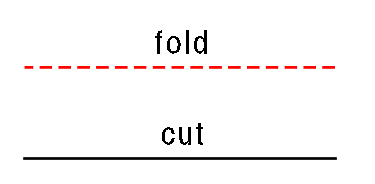
\includegraphics{figures/33_UI_Interface_Data_Structures/foldvsedge.pdf}
\caption{In Foldlings, cuts are displayed as solid black lines. Folds
are displayed as dotted red lines. This convention is familiar to those
who use traditional instructional books
(\citet{berenson1972kirigami},3).}
\end{figure}

An edge represents a cut or fold. Edges are the basic building block of
planes, and an integral element of all fold features. An edge is
minimally defined by a start point, end point, and a a type (either cut
or fold). This minimal definition represents a straight edge between two
points. In addition, an edge can contain further information: the bezier
path drawn to create it (for non-straight edges), and a reference to the
plane or feature it is a part of. Additionally, each edge contains a
reference to its ``twin'' edge.

\subsubsection{Twin Edges}\label{twin-edges}

Although it is often simplest to think of edges as cuts and folds
created by the user, the reality in Foldlings is slightly more
complicated. For each edge that the user creates using a tool, two edges
are created. We create edges with direction, such that there is an edge
from the start point to the end point of the edge, and another edge
starts at the endpoint and has the reverse path of the original edge.
This distinction is most important when detecting planes from edges, but
must also be taken into account whenever edges are processed
(\citet{mallen}). For example, when drawing the 2D view of a sketch, we
skip drawing the twins of edges already drawn, which reduces drawing
work by half.

\begin{figure}[htbp]
\centering
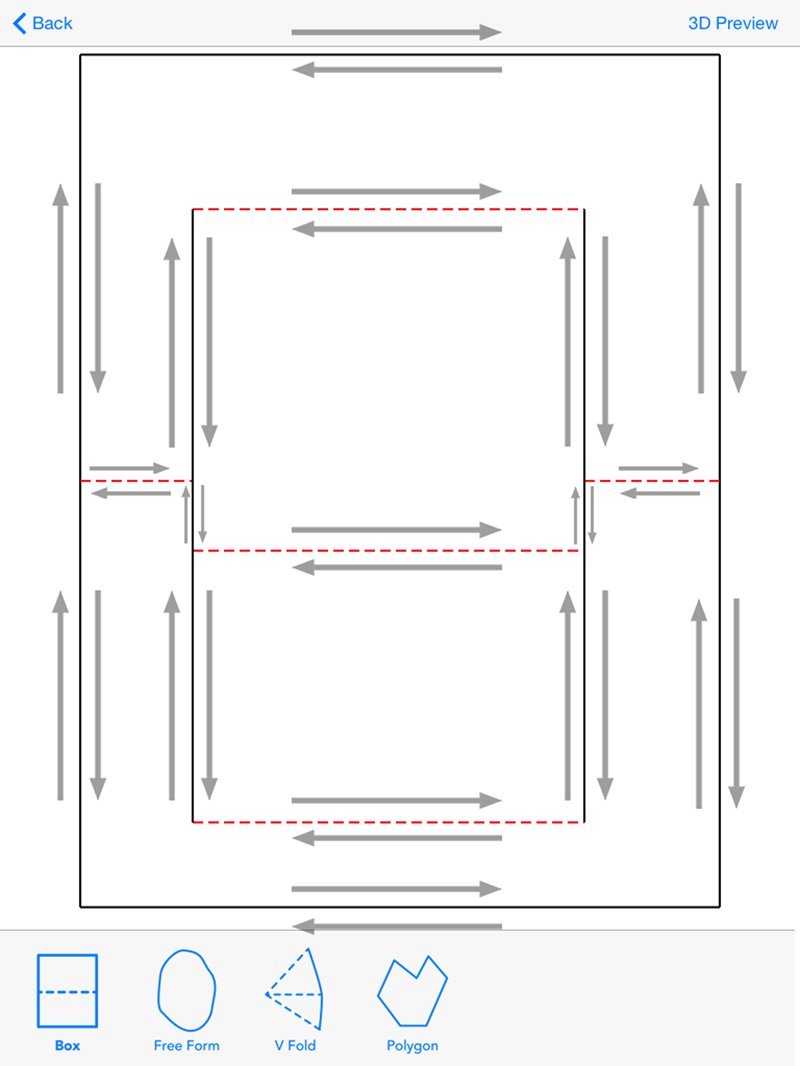
\includegraphics{figures/33_UI_Interface_Data_Structures/boxfold_34_edges.png}
\caption{This sketch contains 34 edges, with orientations shown by the
overlaid gray arrows.}
\end{figure}

\subsubsection{Driving Folds}\label{driving-folds}

\begin{figure}[htbp]
\centering
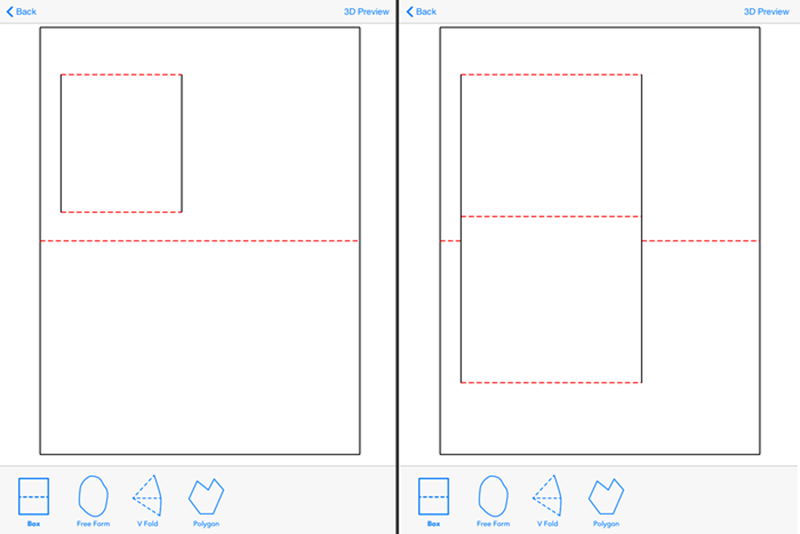
\includegraphics{figures/33_UI_Interface_Data_Structures/boxfold_driving_non_driving.png}
\caption{Left: a box fold mid-drag. The feature does not have a driving
fold. Right: a box-fold after the user has released the touch. The
feature's driving fold is the master card's middle horizontal fold.}
\end{figure}

A driving fold is not a special type of edge, but rather a relationship
between an edge in one feature and a feature ``spanning'' that edge. A
feature is said to span a fold when it is drawn on top of an existing
fold, so that it has horizontal folds both above and below the fold it
spans ---~as shown in figure 1.12.

An edge can be the driving fold for more than one feature, but each
feature has only one driving fold (if there are multiple potential
driving edges at the same height, the leftmost edge is selected). The
driving fold is important for calculating parent-child relationships
between features: a feature's parent is the feature that contains it's
driving fold\footnote{The exception to this rule is holes ---~a hole's
  parent is the feature that contains it.}. These parent-child
relationships are described in more detail in the Chapter \ref{} section
\nameref{nested-features} on page \pageref{nested-features}.
\textbf{\textgreater{}\textgreater{}TODO: FIX BROKEN REF}

\subsubsection{Fold Orientation}\label{fold-orientation}

\begin{figure}[htbp]
\centering
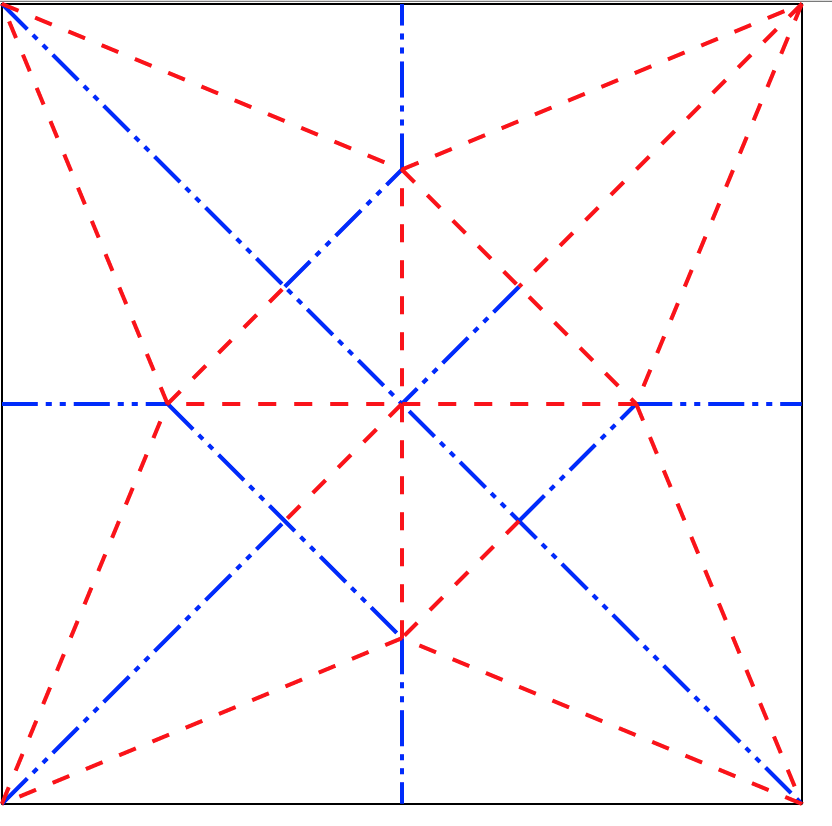
\includegraphics{figures/33_UI_Interface_Data_Structures/maekawas-theorem.png}
\caption{Kirigami fold pattern (\citet{maekawas-theorem}).}
\end{figure}

Traditionally, kirigami patterns indicate direction for folds:
``mountain/hill'' or ``valley''. These folds form angles in opposite
directions ---~mountain folds are pinched away from the paper surface,
while valley folds are pinched into the surface.
\textbf{\textgreater{}\textgreater{}TODO: CITE A BOOK} In Foldlings,
edge orientations are determined by iterating through the plane tree
structure described by \citet{mallen}.

\subsection{Planes}\label{planes}

Planes are an enclosed shape, bounded by edges. Plane are detected from
edges by traversing the directed edge graph, as described in
\citet{mallen}. They are drawn as colored areas in the two-dimensional
sketch, and simulated in the 3D preview as extruded shapes that rotate
about a pivot point. In order to simulate the planes in 3D, we construct
parent-child relationships between the planes, which determine how they
move during simulation.

\begin{figure}[htbp]
\centering
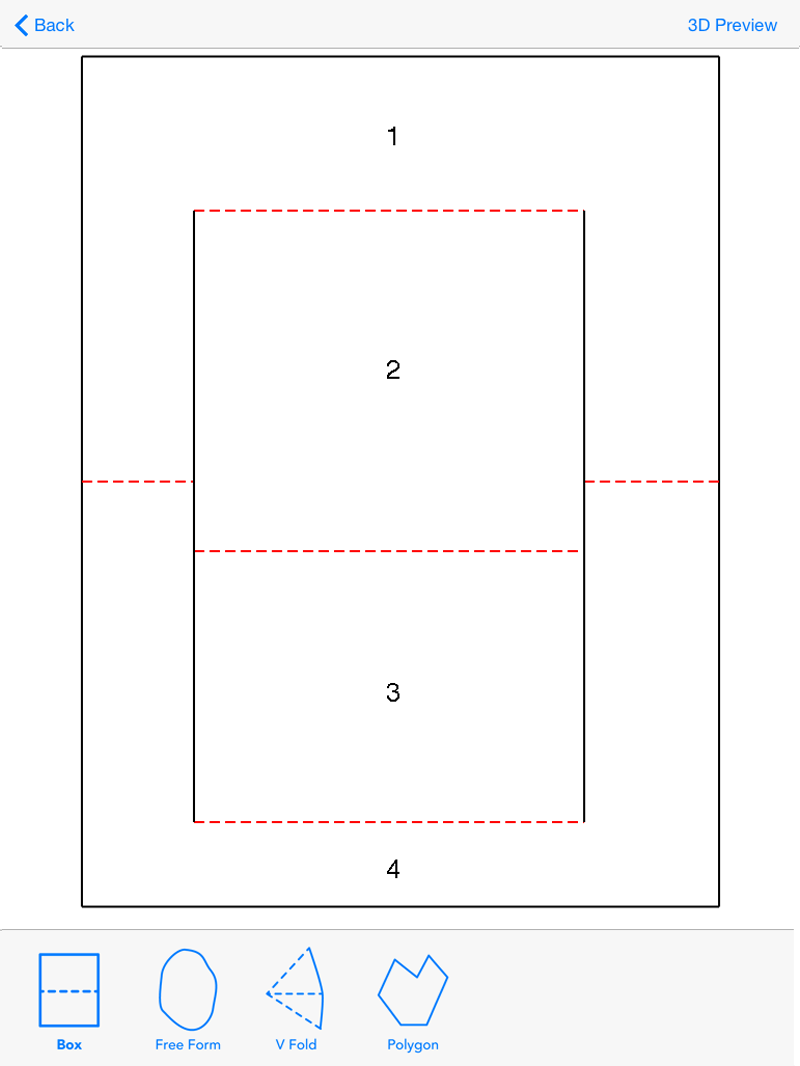
\includegraphics{figures/33_UI_Interface_Data_Structures/boxfold_planes.png}
\caption{Planes in a simple sketch, numbered by ancestry. Starting at
the root plane 1, each successive plane is the child of the previous
numbered plane.}
\end{figure}

\begin{figure}[htbp]
\centering
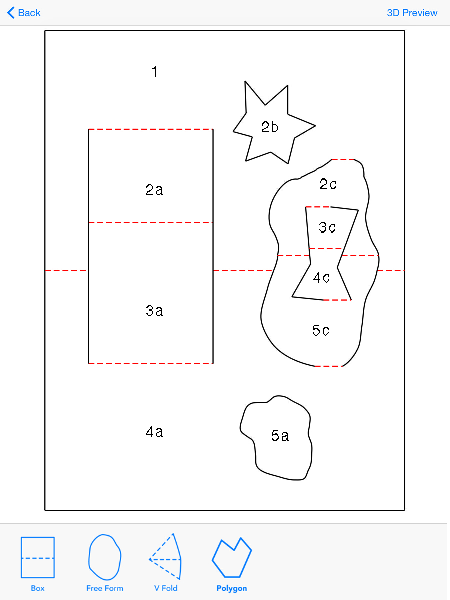
\includegraphics{figures/33_UI_Interface_Data_Structures/complex_sketch.pdf}
\caption{Planes in a more complex sketch, numbered by ancestry. Starting
at the root plane 1, each successive plane is the child of the previous
numbered plane. Letters indicate branches within the plane tree (I.e. 3a
is the child of 2a.}
\end{figure}

\subsection{Fold Features}\label{fold-features}

The central data structure of Foldlings is the fold feature: a
representation of a shape drawn by the user that folds in 3d. Each fold
feature is a single design element ---~and can be individually created,
modified, and deleted. There are five subclasses of FoldFeature:
MasterCard, BoxFold, FreeForm, Polygon, and V-Fold, representing
differences in drawing behavior, geometry, and (the differences are
described in detail below). Each of these features is a subclass of the
FoldFeature superclass.

All fold features have functionality in common:

\begin{itemize}
\itemsep1pt\parskip0pt\parsep0pt
\item
  Each feature contains a list of edges in the feature ---~cuts and
  folds, including twins.
\item
  Each feature has a driving fold --- in the case of unconnected
  features, such as the master card and holes, the driving fold is nil.
\item
  Each feature can be deleted from the dketch, ``healing'' the sketch by
  closing gaps left in any existing cuts and folds.
\item
  Features implement apples \emph{NSEncoding} protocol, allowing them to
  be serialized to a file on the device and restored from the saved
  file.
\item
  Each feature can provide a list of current ``tap options'' --- actions
  that can be performed on the feature given its state.
\item
  Each feature can perform hit-testing: given a point, it can determine
  whether that point is inside or outside the feature.
\end{itemize}

\subsubsection{Master Card}\label{master-card}

Each sketch always contains a single master feature, which is the
ancestor of all other features. It is a simplification of the box fold,
in that it contains three horizontal folds with connecting vertical
cuts. Users do not create features of this type~--- each sketch begins
with one. All of the edges in the master feature are marked with a flag
indicating that they belong to the master feature, because master
feature edges and planes are sometimes treated differently than normal
edges. For example, the parent-child relationships between planes are
constructed by starting at the top plane in the master feature,
determined by edge type and height.

\begin{figure}[htbp]
\centering
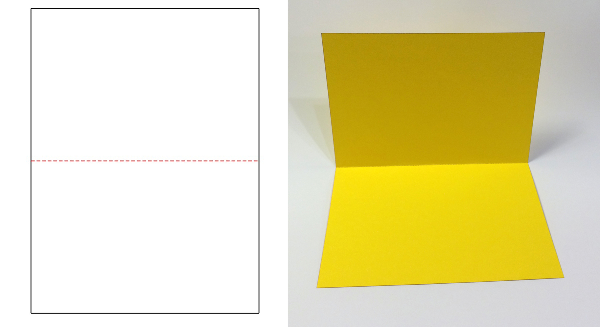
\includegraphics{figures/33_UI_Interface_Data_Structures/mastercard.pdf}
\caption{Left: fold \& cut pattern of the master feature. Right:
laser-cut model of the same.}
\end{figure}

\subsubsection{Box Fold}\label{box-fold}

A box fold consists entirely of straight edges, and can be constructed
from two points: the top left point, and the bottom right point. The
middle fold position is determined by the position of the driving fold,
as described in section on page
\textbf{\textgreater{}\textgreater{}TODO: REF}. Box folds are only valid
if they span a driving fold.

\begin{figure}[htbp]
\centering
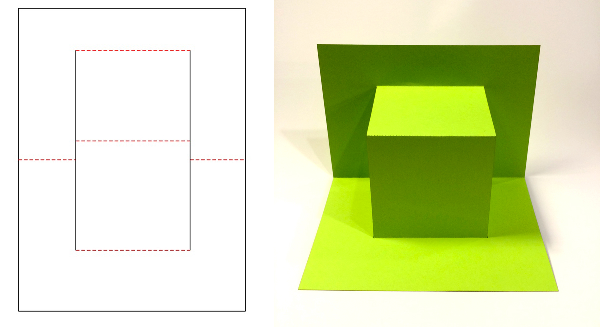
\includegraphics{figures/33_UI_Interface_Data_Structures/box.pdf}
\caption{Left: fold \& cut pattern of the master feature. Right:
laser-cut model of the same.}
\end{figure}

\subsubsection{Free Form}\label{free-form}

Freeform shapes are defined by a single, closed path. When the feature
is completed (by releasing the touch), the shape is truncated,
horizontal folds are added, and the path is split into multiple edges
(assuming the shape spanned a fold\footnote{\textbf{\textgreater{}\textgreater{}TODO:SEE
  SECTION}}). The curved path is defined by a set of ``interpolation
points'' ---~points captured by sampling touch positions while a user
draws a shape on the screen. A path is interpolated between these points
using the Catmull-Rom algorithm (\citet{catmull1974class}).

Holes are a special case of FreeForm shapes, and are cut out from the
final design, rather than simulated as a separate plane. FreeForm shapes
that do not cross a fold are considered holes ---~drawn in white in the
2d sketch and drawn as subtractions from planes in the 3d view.

\begin{figure}[htbp]
\centering
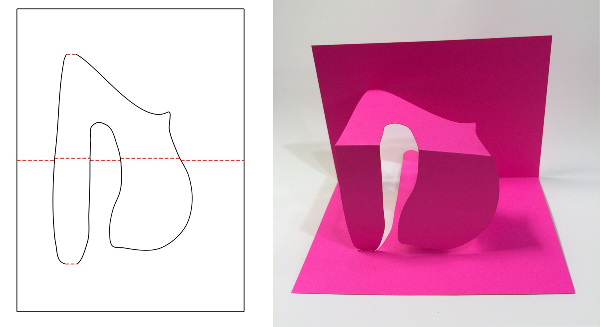
\includegraphics{figures/33_UI_Interface_Data_Structures/free.pdf}
\caption{Left: fold \& cut pattern of a freeform feature. Right:
laser-cut model of the same.}
\end{figure}

\subsubsection{Polygon}\label{polygon}

Polygons are created from a list of ``tap points'' constructed from user
input. As in free-form shapes, these points are connected with a bezier
path, and are truncated if they have a driving fold when they are
completed. For polygons, this path consists only of straight line
segments. Unlike interpolation points, tap points can be moved at any
time during the drawing process.

Like freeform shapes, polygons that do not have a driving fold are
considered holes.

\begin{figure}[htbp]
\centering
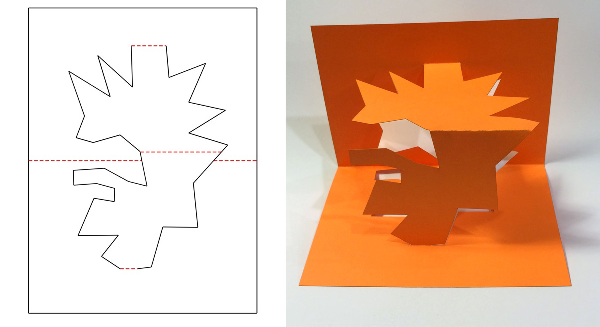
\includegraphics{figures/33_UI_Interface_Data_Structures/poly.pdf}
\caption{Left: fold \& cut pattern of a polygon feature. Right:
laser-cut model of the same.}
\end{figure}

\subsubsection{V-Fold}\label{v-fold}

\begin{figure}[htbp]
\centering
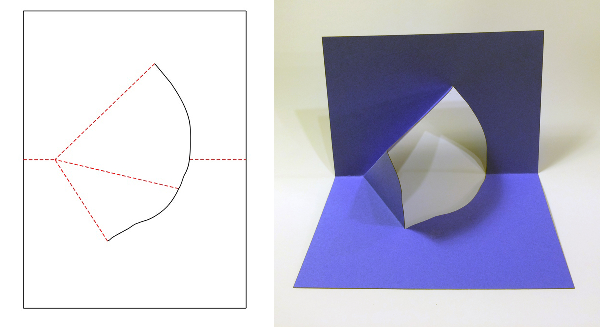
\includegraphics{figures/33_UI_Interface_Data_Structures/v.pdf}
\caption{Left: fold \& cut pattern of a v-fold feature. Right: laser-cut
model of the same.}
\end{figure}

V-folds are partially defined by a path that crosses the driving fold,
called a ``vertical cut.'' This path can be an arbitrary shape that
crosses the driving fold once. They are fully-defined by adding a point
on the driving fold. From this point, we construct three diagonal folds,
two to the top and bottom of the vertical cut, and one to a point that
intersects with the vertical cut at a point calculated to make a valid
90-degree feature \footnote{See Geometric Contraints
  \textbf{\textgreater{}\textgreater{}TODO: REF}}.

\begin{figure}[htbp]
\centering
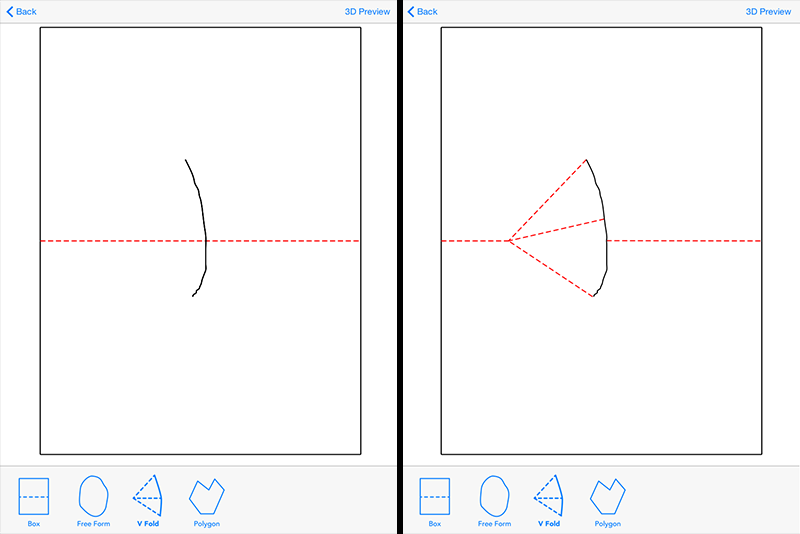
\includegraphics{figures/33_UI_Interface_Data_Structures/vfold_before_after.png}
\caption{Left: an unfinished v-fold, consisting only of a vertical cut.
Right: a v-fold after defining the point on the driving fold to create
diagonal cuts.}
\end{figure}

V-folds are only valid if they have a driving fold, and their vertical
cut intersects the driving fold exactly once.

\subsubsection{Hierarchy}\label{hierarchy}

Fold features have two types of hierarchy. The first is feature
hierarchy: each feature can have other features as children. When a
feature is drawn spanning a fold, its driving fold is set as the fold it
spans, and its parent is the feature that contains this driving fold.
Feature hierarchy allows us to consider each feature individually or as
a chain of features. For actions that only affect a single feature, we
need only consider the edges in the feature and it's driving fold. We
can also traverse the tree to perform actions on a chain of features.
The second type of hierarchy is parent-child relationships between
planes. Each plane has one or more children, forming a branching tree
that starts at the top plane of the master card and ends with the master
card's bottom plane as one of its leaf nodes. This hierarchy is
described in \textbf{\textgreater{}\textgreater{}TODO: REF}, and is most
important for rendering the scene in 3D.

\subsection{Sketches}\label{sketches}

A sketch is the representation of the user's drawing ---~its primary
role is as a collection of features. It also contains information about
the current drawing state, and the state of user interaction (for
example, which features are currently being modified, and which tool is
selected).
